\subsubsection{Erstellen eines Patches}

Um einen Patch zu erstllen selektieren Sie im Package bzw. Project Explorer die beiden Modelle zwischen denen die asymmetrische Differenz berechnet werden soll.
Öffnen Sie mit der rechten Maustaste das Kontextmenü und wählen Sie \texttt{SiLift} $\triangleright$ \texttt{Create a Patch} aus (vgl. Abb. \ref{silift-tutorial_patching_contextmenu_create}).

\begin{figure}[H]
\centering
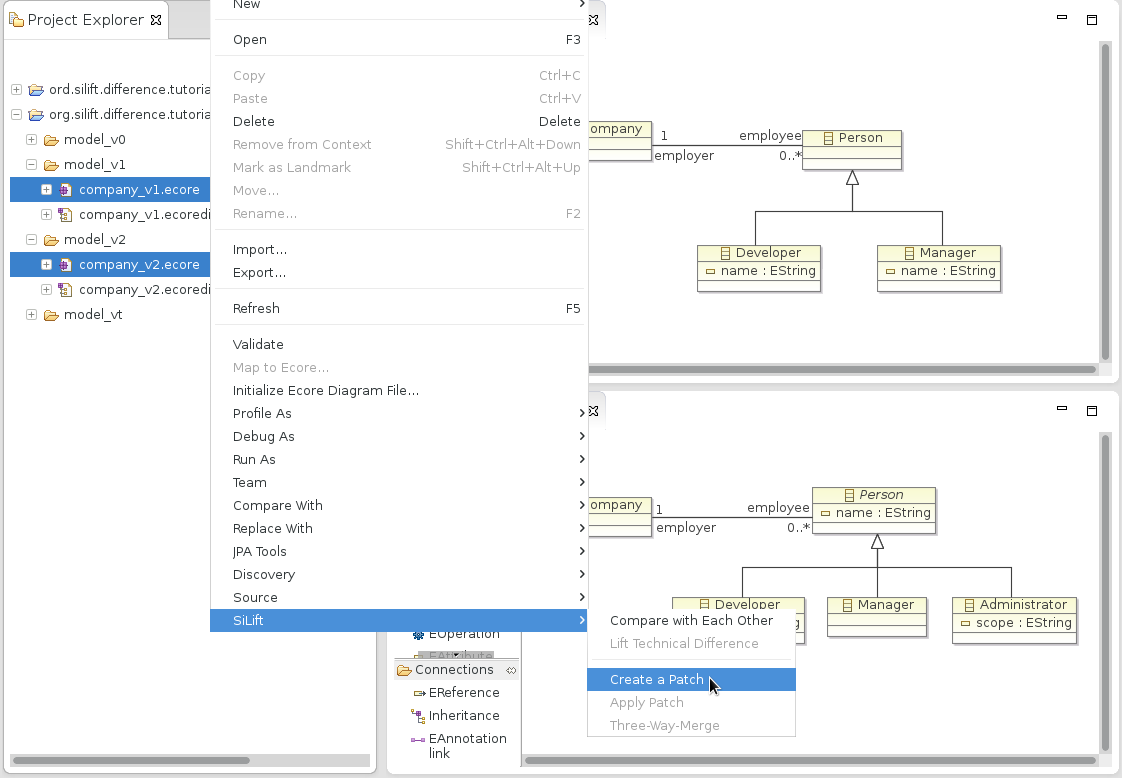
\includegraphics[width=0.8\textwidth]{patching/graphics/silift-tutorial_patching_contextmenu_create.png}
\caption{SiLift: Patch erstellen}
\label{silift-tutorial_patching_contextmenu_create}
\end{figure}

Es öffnet sich ein neues Fenster, welches analog zu Abbildung \ref{silift-wizard_compare_page1} mehrere Konfigurationsmöglichkeiten bietet (vgl. Abb. \ref{silift-tutorial_patching_create_config}).


\begin{figure}[H]
\centering
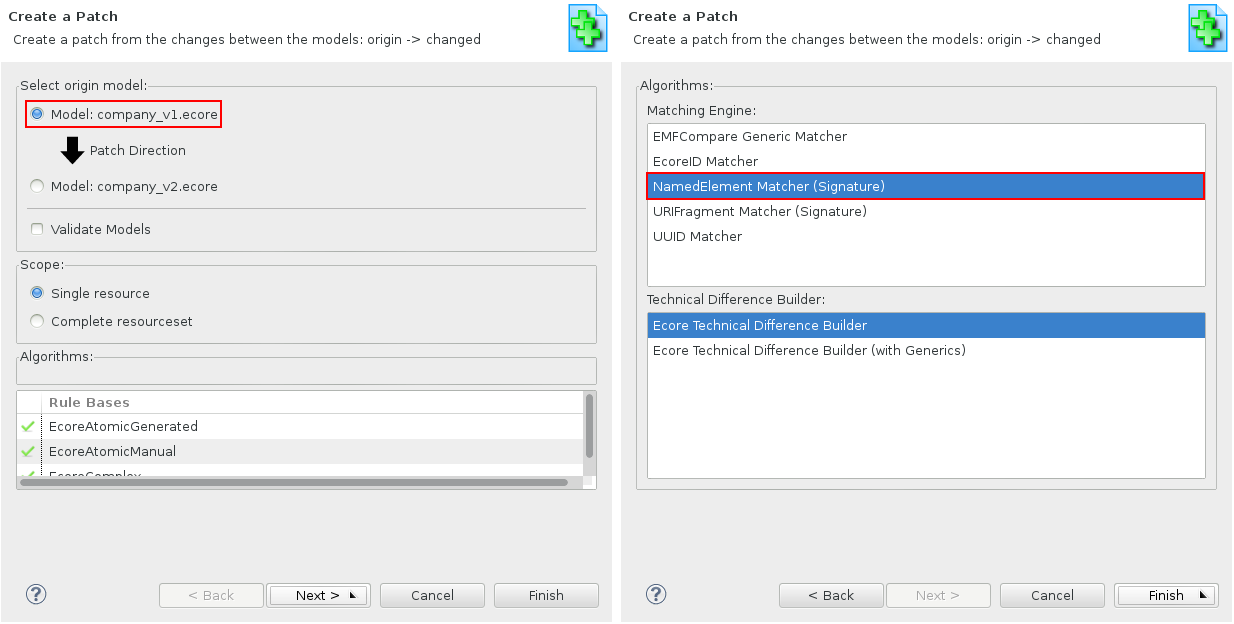
\includegraphics[width=0.8\textwidth]{patching/graphics/silift-tutorial_patching_create_config.png}
\caption{Patch-Config}
\label{silift-tutorial_patching_create_config}
\end{figure}

Nach erfolgreicher Generierung wird der Patch im Ordner des Basismodells gespeichert und in einem entsprechenden Editor geöffnent.
Dieser bietet die Möglichkeit einen Patch nachträglich noch zu bearbeiten, indem einzelne Editieroperationen deaktiviert werden können (vgl. Abb. \ref{silift-tutorial_patching_modify_patch}).

\begin{figure}[H]
\centering
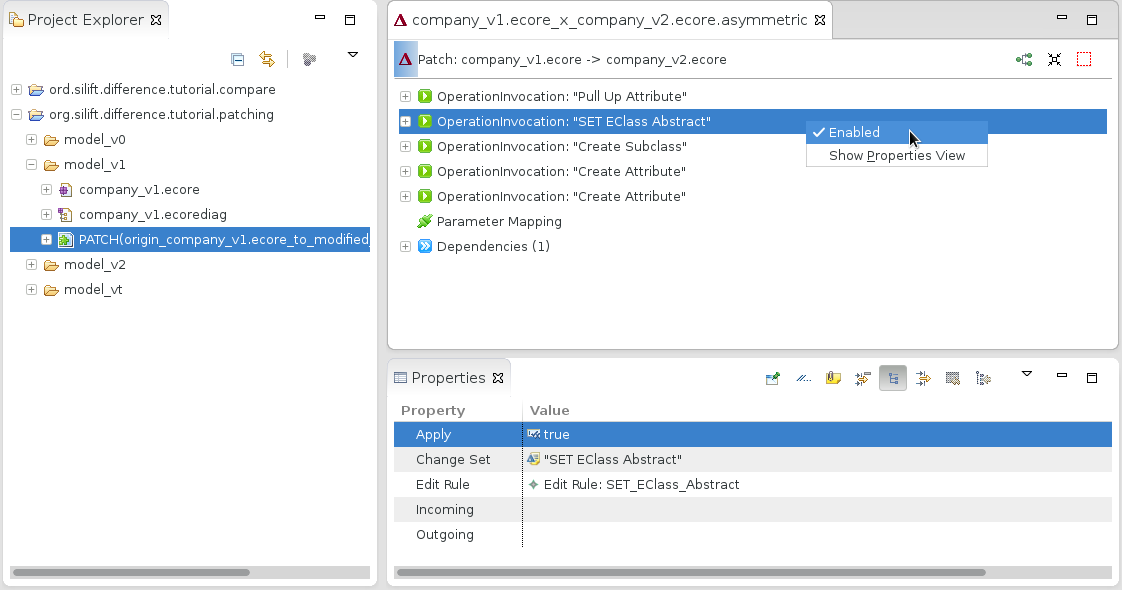
\includegraphics[width=0.8\textwidth]{patching/graphics/silift-tutorial_patching_modify_patch.png}
\caption{Patch-Editor}
\label{silift-tutorial_patching_modify_patch}
\end{figure}